%%%%%%%%%%%%%%%%%%%%%%%%%%%%%%%%%%%%%%%%%%%%%%%%%%%%%%%%%%%%%%%%%%%%%%%%%%%%%%%%%%%%%%
% Key Concept II       
%%%%%%%%%%%%%%%%%%%%%%%%%%%%%%%%%%%%%%%%%%%%%%%%%%%%%%%%%%%%%%%%%%%%%%%%%%%%%%%%%%%%%%
\section{Key Concept II \tiny Nebenläufige Prozesse und Prozessiteration}

\subsection{Signale}

\begin{minipage}{0.01\textwidth}
	\text{ } %platzhalter
\end{minipage}
\begin{minipage}{0.48\textwidth}
	\begin{VHDL}
--  Definition 
signal <signal_name1> {,<signal_name2>}: <singal_type> [:= initial_value]
-- Std zuweisung
y <= x;
-- Unbedingte Signalzuweisung 
[label:] <signal_name> <= Expression {, Exression};
Y <= '1'; ["100101";] [A and B;]	-- Beispiele
	\end{VHDL}
\end{minipage}
\begin{minipage}{0.02\textwidth}
	\text{ } %platzhalter
\end{minipage}
\begin{minipage}{0.48\textwidth}
	\begin{VHDL}
-- Selektive Signalzuweisung
[label:] with <select_signal> select
	<dest_sig> <= 	{surce_sig_1 when select_value_1,}
					source_sig_n when others;
-- Bedingte Signalzuweisung
[label:] <dest_sig> <=	{expr_1 when condition_1 else}
						expr_n
	\end{VHDL}
\end{minipage}

\subsection{Nebenläufigkeit Prozesse}

\begin{minipage}{0.01\textwidth}
	\text{ } %platzhalter
\end{minipage}
\begin{minipage}{0.35\textwidth}
	\begin{VHDL}
--  Definition 
[<label:] process [(<Sensitivitaetsliste>)] -- falls keine, wait nicht vergessen
	<Deklarationsteil> -- Prozess intern
begin 
	{<sequentielle Anweisungen>}
end process [<lable>];
-- nur Variabeln im Prozesses aenderbar Bsp.
variable <var_name>: <type> [ := expr]; 
	\end{VHDL}
\end{minipage}
\begin{minipage}{0.02\textwidth}
	\text{ } %platzhalter
\end{minipage}
\begin{minipage}{0.26\textwidth}
	\begin{VHDL}
-- sequenzielle Anweisungen - if
if condition_a then 
	{sequential statements};
{elsif condition_b then
	{sequential statements};}
else 
	{sequential statments};
end if;

	\end{VHDL}
\end{minipage}
\begin{minipage}{0.02\textwidth}
	\text{ } %platzhalter
\end{minipage}
\begin{minipage}{0.32\textwidth}
	\begin{VHDL}
-- case
case expression is 
	when choice_1 	=> {sequential statement};
	{when choice_n	=> {sequential statement};}
	when others	  	=> {sequential statement};
end case;
	\end{VHDL}
\end{minipage}


\subsection{Sequentielle Schaltung}

\begin{minipage}{.5\textwidth}
	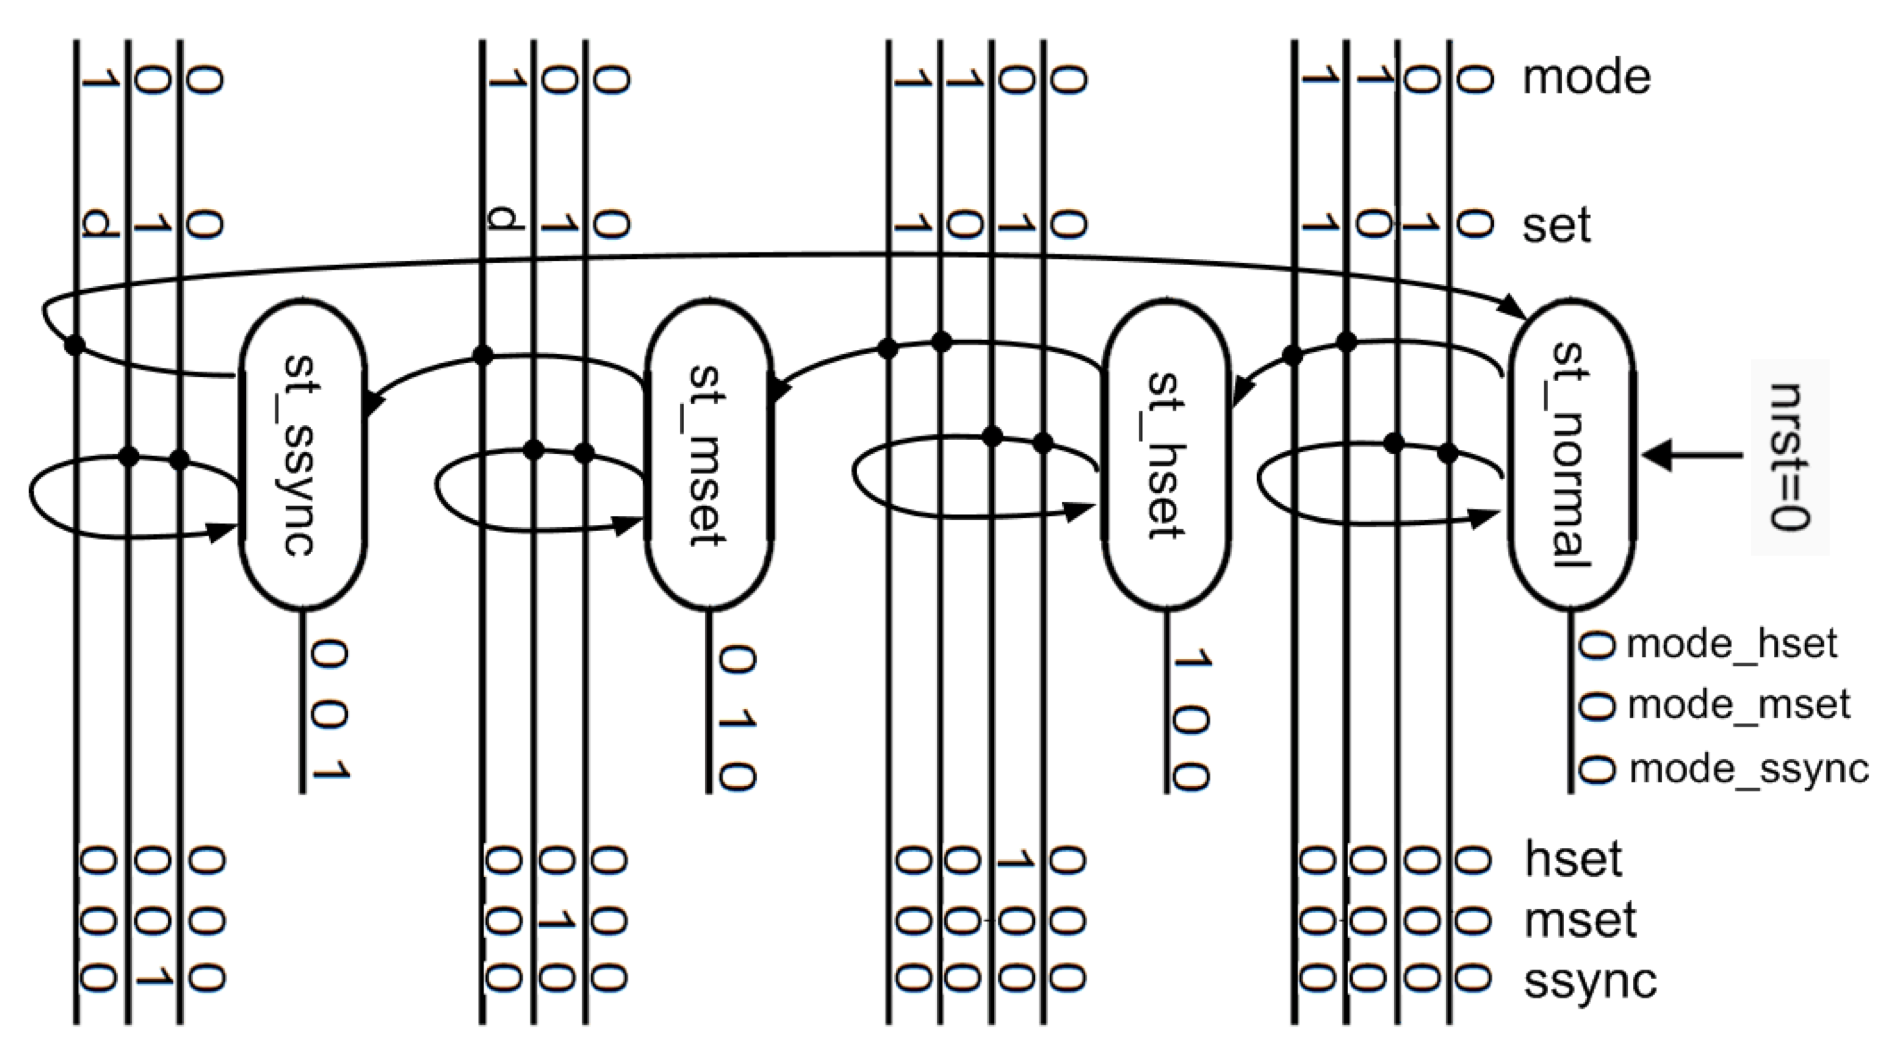
\includegraphics[width=\textwidth]{./bilder/ZDiagramm}
\end{minipage}
\begin{minipage}{0.02\textwidth}
	\text{ } %platzhalter
\end{minipage}
\begin{minipage}{.48\textwidth}
	$\cdot$ FSM ähnliche Zustände wie Z-Diagramm\\
	$\cdot$ empfohlen die Übergänge mit einem CLK zu lösen
	\begin{VHDL}
if CLK'event and (CLK = '1') then {} -- pos falnke ('0' neg) \end{VHDL}

	$\cdot$ Signale in synchronem Prozess auf linker Seite -> FF{\tiny Flip-Flop} \\
	$\cdot$ in Sensitivitätsliste nur CLK (und RST)\\
	$\cdot$ if Anweisungen mit CLK immer am Schluss des Prozesses\\
	$\cdot$ Aufzählungstyp (z.B. für Prozessname) {\tiny  Anzahl Bits kann auch defieniert werden}
	\begin{VHDL}
type <enum_type_name> is (type_element{, type_element});	\end{VHDL}
	$\cdot$ hinterlegte Bits für Aufzählungstyp selber bestimmen
	\begin{VHDL}
attribute <ENUM> : <ENUM_type>;	-- ENUM encoding
attribute <ENUM> of	<aufz_type> : type is expression
subtype <aufz_type> is <const_type>; -- constant encoding
constant <aufz_type_element> : <aufz_type> := expression  \end{VHDL}
\end{minipage}

\subsection{Endliche Z-Maschinen}

\begin{minipage}{.6\textwidth}
	\begin{VHDL}
-- Prozess G = next_state_logic: Kombinatorischer Prozess
	next_state_logic: process (INP, present_state)
	begin 
		{Kombinatorische Anweisungen} -- Bestimmung des next_state
	end process;
	
-- Prozess Z = state_register:
	state_register: process (CLK, RST)
	begin 
		{Sequentielle Anweisungen} -- Aktualisiert bei CLK den present_state
	end process;
 
-- Prozess F = Output_Logic: 1. Mealy
	output_logic: process (INP, present_state)
	begin
		{output_bestimmung} -- Ausgang von IMP und present_state abhaengig
	end process
-- 2. Moore
	output_logic: process (present_state)
	begin
		{output_bestimmung} -- Ausgang nur vom present_state abhaengig
	end process
-- 3. Medwedjew
	output_logic: OUP <= present_state;
	\end{VHDL}
\end{minipage}
\begin{minipage}{.4\textwidth}
	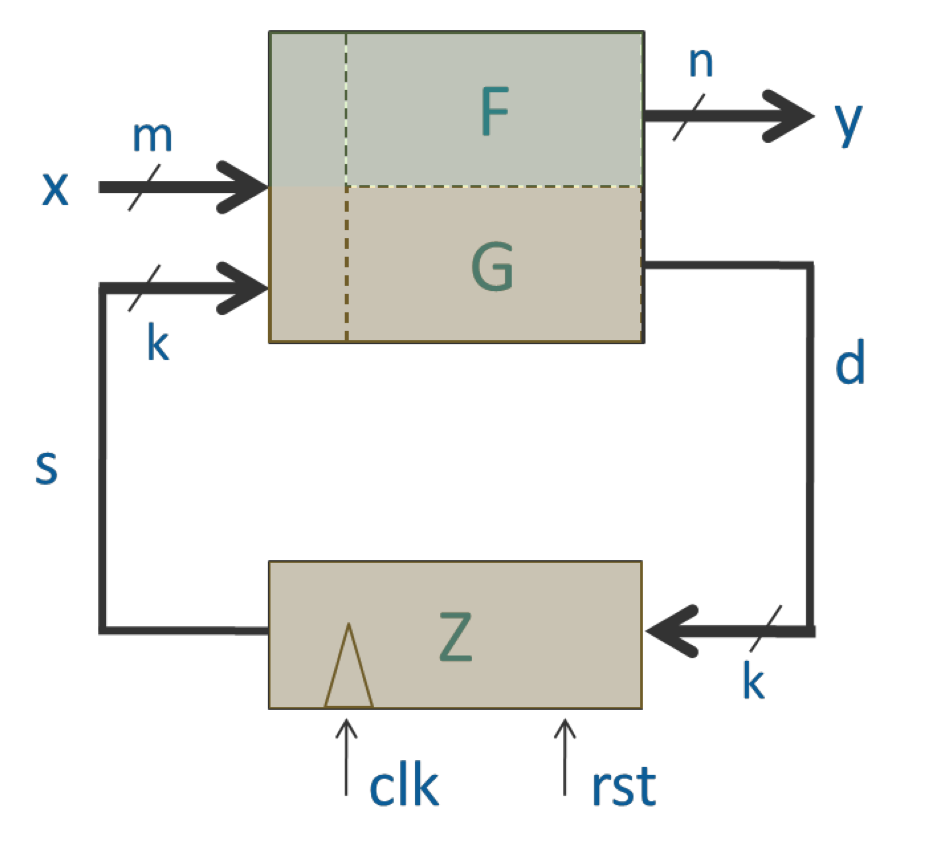
\includegraphics[width=\textwidth]{./bilder/ZMaschiene}
\end{minipage}
